\chapter{Vacuum Energy, Expansion, and de Sitter Horizons}

These notes follow Leonard Susskind's eighth lecture in the supplementary \emph{Cosmology and Black Holes} track, keeping the order in which the lecture itself unfolds. The lecture does not begin with horizons. It begins with student questions about vacuum energy, then explains why vacuum energy is unlike ordinary matter, then inserts it into Einstein's equations, and only after that turns to accelerated expansion and event horizons. The aim here is to preserve that progression while writing the mathematics in a clean form. These notes are presented as a companion to Leonard Susskind's lecture and are curated by LazyingArt LLC.

\section{Vacuum Energy and Why It Is Special}

The lecture opens with a question about whether virtual electron--positron pairs are ``really'' produced in the vacuum. Susskind's answer is careful: virtual processes contribute to the energy of the vacuum, but they are not ordinary observable particles flying out of empty space. His first concrete model is the harmonic oscillator. Classically the oscillator can sit motionless at the bottom of its potential, but quantum mechanically the ground state still carries energy:
\begin{equation}
E_{\text{ground}}=\frac{1}{2}\hbar\omega.
\end{equation}
This is the first mathematical anchor for the lecture's notion of vacuum energy. The electromagnetic field in a cavity can be viewed as a collection of harmonic oscillators, each with its own zero-point energy. Summing those zero-point contributions produces a vacuum energy density.

The lecture then pivots to the more subtle question: if empty space contains positive energy density, why does it not behave like a material medium and slow light down? Susskind's answer is that ordinary matter and vacuum energy are not the same kind of thing. Ordinary matter picks out a preferred rest frame. Vacuum energy does not. It is the special form of energy whose measured density is the same for every inertial observer. In the language used later in the lecture, if we denote the vacuum energy density by \(\rho_{\rm vac}\), then
\begin{equation}
\rho_{\rm vac}=\text{const.}
\end{equation}
not only in time for an expanding universe, but also with respect to the state of motion of the observer.

That point is the real beginning of the cosmology discussion. Vacuum energy is not merely ``energy in the vacuum.'' It is the unique energy density that does not define a preferred Lorentz frame. That is why Susskind treats it as compatible with the local statement that light moves with speed \(c\) in empty space.

\section{Einstein's Equations and a Very Special Geometry}

So long as gravity is ignored, the zero of energy is often unimportant. The lecture emphasizes that gravity changes this. Gravity couples to energy, and therefore vacuum energy cannot be dismissed once one is asking about spacetime geometry.

Susskind first reminds the audience of the schematic structure of Einstein's equations. The left-hand side is geometric, built from the metric tensor \(g_{\mu\nu}(x)\), and the right-hand side is the energy-momentum content of matter and fields. In standard notation one may write this schematically as
\begin{equation}
G_{\mu\nu}\propto T_{\mu\nu},
\end{equation}
where the proportionality constant is not the point of this stage of the lecture. The important point is the division into geometry on the left and material source on the right.

\begin{figure}[htbp]
\centering

\includegraphics[width=0.58\textwidth]{lecture_08_figure_02.png}
\caption{Documentary board state at the moment Susskind identifies \(G_{\mu\nu}\) as the geometric side of Einstein's equations and writes the underlying metric notation \(g_{\mu\nu}(x)\).}
\end{figure}

He then narrows immediately to a very special spacetime geometry: spatially flat space expanding uniformly in time. In the board notation preserved in the lecture frames, the metric is written as
\begin{equation}
ds^2=-dt^2+a(t)^2\,dx^2.
\end{equation}
Here \(dx^2\) is shorthand for the Euclidean spatial piece \(dx^2+dy^2+dz^2\). The function \(a(t)\) is the scale factor. The coordinate separation \(\Delta x\) between two marked points on the ``rubber sheet'' is fixed, while the physical separation grows with the scale factor:
\begin{equation}
D_{\rm phys}(t)=a(t)\,\Delta x.
\end{equation}
This is exactly the simplified setup Susskind wants: once the geometry has been reduced to this ansatz, Einstein's equations become equations for the time dependence of \(a(t)\).

\section{The Friedmann Equation, Matter Dilution, and a Worked Solution}

For the spatially flat metric above, the lecture writes Einstein's equations in the form
\begin{equation}
\left(\frac{\dot a}{a}\right)^2=\frac{8\pi G}{3}\rho(t),
\end{equation}
with \(\rho(t)\) the homogeneous energy density filling the universe.

\begin{figure}[htbp]
\centering

\includegraphics[width=0.86\textwidth]{lecture_08_figure_04.png}
\caption{The clearest surviving board frame for the metric \(ds^2=-dt^2+a(t)^2dx^2\) and the corresponding Friedmann equation \(\left(\dot a/a\right)^2=(8\pi G/3)\rho(t)\).}
\end{figure}

The lecture then asks what \(\rho(t)\) actually does for ordinary matter. The answer is derived from a comoving box argument rather than simply quoted. Take a box with fixed coordinate side \(\Delta x\). Its physical side length is \(a(t)\Delta x\), so its physical volume is \(a(t)^3(\Delta x)^3\). If the box contains \(n\) nonrelativistic particles of mass \(m\), then
\begin{equation}
\rho_m(t)=\frac{nm}{a(t)^3(\Delta x)^3}.
\end{equation}
Choosing \((\Delta x)^3=1\) for convenience, one can write
\begin{equation}
\rho_m(t)=\rho_0\,a(t)^{-3}.
\end{equation}
This is the first major contrast with vacuum energy. Ordinary matter dilutes as the universe expands.

\paragraph{Worked derivation of the matter-dominated solution.}
Substituting \(\rho_m(t)=\rho_0 a^{-3}\) into the Friedmann equation gives
\begin{align}
\left(\frac{\dot a}{a}\right)^2&=\frac{8\pi G}{3}\frac{\rho_0}{a^3}.
\end{align}
Absorb the constant \((8\pi G/3)\rho_0\) into a single positive constant \(K\). Then
\begin{align}
\left(\frac{\dot a}{a}\right)^2&=K a^{-3},\\
\dot a^2&=K a^{-1}.
\end{align}
Taking the expanding branch,
\begin{equation}
\dot a=\sqrt{K}\,a^{-1/2}.
\end{equation}
Now separate variables:
\begin{equation}
a^{1/2}\,da=\sqrt{K}\,dt.
\end{equation}
Integrating both sides yields
\begin{equation}
\frac{2}{3}a^{3/2}=\sqrt{K}\,t+\text{constant}.
\end{equation}
Discarding irrelevant normalization constants, the result is
\begin{equation}
a(t)\propto t^{2/3}.
\end{equation}

This is Susskind's matter-dominated cosmology. The expansion is not linear in time. It decelerates. The lecture's physical interpretation is simple: things started out moving apart, and gravity slows the expansion down.

The lecture briefly remarks that radiation behaves differently:
\begin{equation}
\rho_{\rm rad}(t)\propto a(t)^{-4},
\end{equation}
but does not work out that branch in detail here.

\paragraph{A lecture-specific heuristic about energy conservation.}
At this point Susskind pauses over a useful but potentially misleading reformulation. He reads the Friedmann equation as if it were a balance between positive matter energy and a negative gravitational contribution:
\begin{equation}
-\left(\frac{\dot a}{a}\right)^2+\frac{8\pi G}{3}\rho(t)=0.
\end{equation}
In the lecture this is presented as a way of thinking about the time-dependent gravitational field as carrying a negative contribution to the total energy.

\begin{remark}
This ``minus this plus this equals zero'' reading is faithful to the lecture, but it should be understood as a minisuperspace heuristic for this cosmological ansatz, not as a blanket statement of globally conserved energy in arbitrary expanding spacetimes.
\end{remark}

\begin{figure}[htbp]
\centering

\includegraphics[width=0.82\textwidth]{lecture_08_figure_03.png}
\caption{Intermediate board state from the lecture. The left edges are cropped, but the metric line and the density term in the Friedmann equation are already arranged as the two-line cosmology block that Susskind then interprets heuristically as an energy-balance equation.}
\end{figure}

\section{Vacuum Energy and Exponential Expansion}

The lecture now repeats the analysis with the one energy density that does \emph{not} dilute:
\begin{equation}
\rho(t)=\rho_{\rm vac}.
\end{equation}
Then the Friedmann equation becomes
\begin{equation}
\left(\frac{\dot a}{a}\right)^2=\frac{8\pi G}{3}\rho_{\rm vac}.
\end{equation}
Because the right-hand side is constant, Susskind names it \(H^2\):
\begin{equation}
H^2=\frac{8\pi G}{3}\rho_{\rm vac}.
\end{equation}
At this stage \(H\) is no longer merely the definition \(\dot a/a\); in the pure vacuum case it is also a constant number determined by the vacuum energy density. The evolution equation is therefore
\begin{equation}
\dot a=Ha,
\end{equation}
and its solution is
\begin{equation}
a(t)=C e^{Ht},
\end{equation}
with \(C\) an integration constant fixed by normalization.

This is the central cosmological payoff of the lecture: vacuum energy produces exponential expansion. The distinction from the matter-dominated case is not minor. In the matter-dominated solution, expansion slows. In the vacuum-dominated solution, the rate of change of \(a\) is proportional to \(a\) itself, and the universe accelerates.

The same discussion is recast in Hubble-law language. If recession speed and distance are related by
\begin{equation}
v=HD,
\end{equation}
then in the pure vacuum case the distance at which recession speed equals \(c\) is
\begin{equation}
D_H=\frac{c}{H}.
\end{equation}
Because \(H\) is constant, this distance is constant as well. The lecture does not yet identify this with the full event-horizon story, but it does use it as a first signal that the accelerated universe has a fixed characteristic distance scale.

The physically relevant universe contains more than vacuum energy. It also contains matter, whose density scales like \(a^{-3}\). Thus the lecture's qualitative history is
\begin{equation}
a(t)\sim t^{2/3}\qquad\text{early on},
\end{equation}
followed at late times by
\begin{equation}
a(t)\sim e^{Ht}.
\end{equation}
That crossover is exactly what Susskind says cosmological observations seem to show.

\begin{figure}[htbp]
\centering
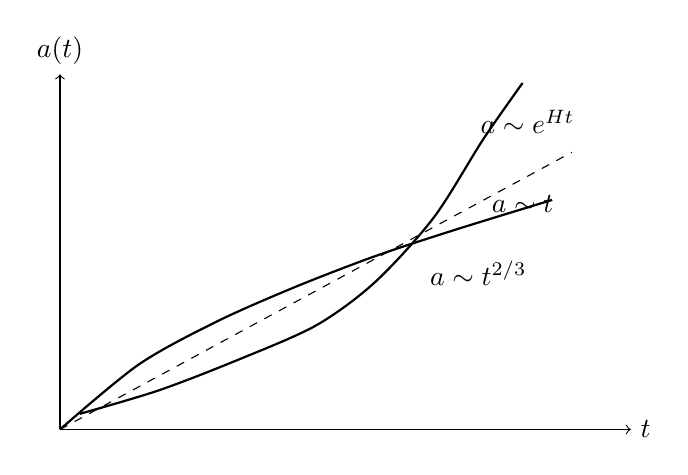
\begin{tikzpicture}[x=1.25cm,y=1.1cm]
\draw[->] (0,0) -- (5.8,0) node[right] {$t$};
\draw[->] (0,0) -- (0,4.1) node[above] {$a(t)$};

\draw[dashed] (0,0) -- (5.2,3.2);
\node at (4.7,2.6) {$a\sim t$};

\draw[thick] plot[smooth] coordinates {(0,0) (0.8,0.75) (1.6,1.25) (2.4,1.65) (3.2,2.0) (4.0,2.3) (5.0,2.65)};
\node at (4.25,1.8) {$a\sim t^{2/3}$};

\draw[thick] plot[smooth] coordinates {(0.2,0.18) (1.0,0.45) (1.8,0.8) (2.6,1.2) (3.2,1.7) (3.8,2.45) (4.3,3.35) (4.7,4.0)};
\node at (4.75,3.55) {$a\sim e^{Ht}$};
\end{tikzpicture}
\caption{Transcript-backed reconstruction of the lecture's qualitative comparison of linear growth, matter-dominated growth, and the late-time exponential takeoff driven by vacuum energy.}
\end{figure}

\section{Bound Systems and the Observational Future}

Before turning to the geometry of horizons, the lecture cashes out the physics of exponential expansion in ordinary language. The important distinction is not between ``things that feel gravity'' and ``things that do not.'' The important distinction is between systems that are gravitationally bound and systems that are merely participating in the Hubble flow.

That is why the lecture treats Andromeda differently from distant galaxies. Nearby bound structures do not get torn apart simply because the universe is accelerating. If two galaxies are already bound, the question is essentially local: are they moving relative to each other with more than escape velocity or not? Distant galaxies that are not bound, by contrast, continue to separate, and in a vacuum-dominated future they eventually leave observational reach.

Susskind also gives a Newtonian-style picture, carefully only as intuition. Ordinary gravitational attraction falls with distance, while the vacuum-energy contribution can be mimicked by a very weak outward effect that grows with distance. The lecture does \emph{not} fix the exact coefficient at this stage, and it is better to preserve that restraint here. The important qualitative point is that the vacuum term matters only on genuinely cosmological distance scales.

The observational future described in the lecture is stark. Matter and radiation dilute away, the vacuum energy remains, and the world becomes increasingly empty. Local bound remnants remain, but galaxies that ride with the cosmological flow eventually disappear across the relevant horizon scale. This is the practical motivation for the horizon discussion that follows.

\section{De Sitter Space, Conformal Time, and Event Horizons}

After the break, the lecture returns to the pure vacuum case and gives the spacetime a name. If
\begin{equation}
a(t)=e^{Ht},
\end{equation}
then the metric becomes
\begin{equation}
ds^2=-dt^2+e^{2Ht}dx^2.
\end{equation}
This is de Sitter space in the flat slicing used throughout the lecture.

Susskind now introduces a new time coordinate \(T\) designed to compress the infinite future into a finite coordinate interval while keeping light rays at \(45^\circ\). The definition is
\begin{equation}
dt^2=e^{2Ht}dT^2,
\end{equation}
or equivalently,
\begin{equation}
dt=e^{Ht}dT.
\end{equation}
Rearranging and integrating,
\begin{align}
e^{-Ht}\,dt&=dT,\\
T&=-\frac{1}{H}e^{-Ht}+ \text{constant}.
\end{align}
By shifting the additive constant, one may choose
\begin{equation}
T=-\frac{1}{H}e^{-Ht}.
\end{equation}
Then \(T<0\), the remote past is \(T\to -\infty\), and the infinite future corresponds to the finite location
\begin{equation}
T\to 0^{-}.
\end{equation}

From \(HT=-e^{-Ht}\) one obtains
\begin{equation}
e^{2Ht}=\frac{1}{H^2T^2},
\end{equation}
so the metric becomes
\begin{equation}
ds^2=\frac{1}{H^2T^2}\left(-dT^2+dx^2\right).
\end{equation}
This is the clean conformal form that the lecture wants. For light rays,
\begin{equation}
ds=0,
\end{equation}
so the overall factor \(1/(H^2T^2)\) drops out and one is left with
\begin{equation}
dT=\pm dx.
\end{equation}
Thus light rays travel on \(45^\circ\) lines in the \((T,x)\) diagram.

\begin{definition}
Given an observer worldline, the event horizon is the boundary separating the region from which signals can reach arbitrarily late points on that worldline from the region that can never do so.
\end{definition}

The lecture motivates this definition by recalling the familiar black-hole story: in flat spacetime a sufficiently late observer can, in principle, see the whole spacetime, whereas in a black-hole spacetime there is a region forever hidden behind the horizon. De Sitter space turns out to have the same causal feature, but now the horizon is not tied to a localized gravitating body. It is a property of the accelerated spacetime itself.

\begin{figure}[htbp]
\centering
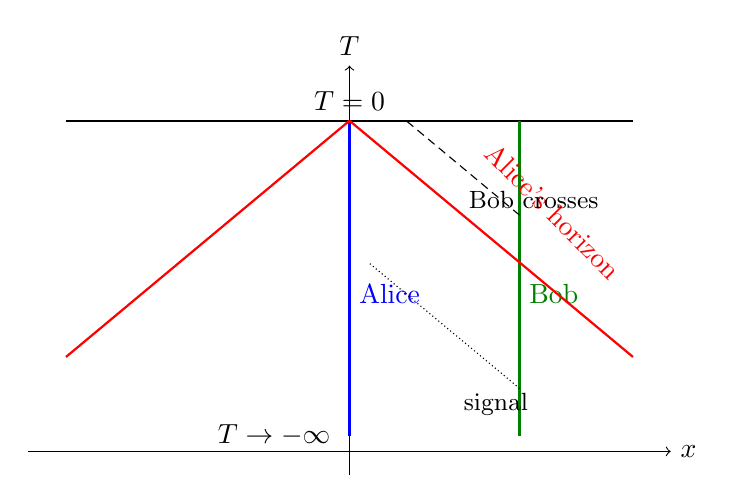
\begin{tikzpicture}[x=1.2cm,y=1.0cm]
\draw[thick] (-3,0) -- (3,0);
\node[above] at (0,0) {$T=0$};

\draw[->] (-3.4,-4.2) -- (3.4,-4.2) node[right] {$x$};
\draw[->] (0,-4.5) -- (0,0.7) node[above] {$T$};
\node[left] at (-0.1,-4.0) {$T\to -\infty$};

\draw[blue,thick] (0,-4) -- (0,0);
\node[blue,right] at (0,-2.2) {Alice};

\draw[green!50!black,thick] (1.8,-4) -- (1.8,0);
\node[green!50!black,right] at (1.8,-2.2) {Bob};

\draw[red,thick] (0,0) -- (3,-3);
\draw[red,thick] (0,0) -- (-3,-3);
\node[red,rotate=-45] at (2.15,-1.15) {Alice's horizon};

\draw[densely dashed] (1.8,-1.2) -- (0.6,0);
\node at (1.95,-1.0) {\small Bob crosses};

\draw[densely dotted] (1.8,-3.4) -- (0.2,-1.8);
\node at (1.55,-3.6) {\small signal};

\end{tikzpicture}
\caption{Cautious transcript-backed reconstruction of the de Sitter conformal diagram used in the lecture. The top edge \(T=0\) is the infinite future in proper time, light rays follow \(45^\circ\) lines, and Alice's past light cone never covers the whole spacetime.}
\end{figure}

This diagram captures the lecture's main causal claim. Alice can wait longer and longer and thereby enlarge the region of spacetime that she has seen, but no amount of waiting allows her to see everything. Bob may have been visible earlier, yet once his worldline passes outside Alice's horizon he can no longer send her a signal. The lecture then adds an important practical refinement: even when a signal is formally still arriving from very near the horizon, it becomes extremely redshifted. Causal disappearance and observational disappearance come together.

A final subtle point in the lecture is that the proper distance to the horizon stays fixed. In conformal coordinates the coordinate distance to the horizon shrinks, but the conformal factor grows, and the two effects balance. That constancy is the geometric version of the earlier statement that \(H\) remains constant in the pure vacuum case.

\section{Summary}

The lecture's chain of ideas is tight. Vacuum energy begins as zero-point energy and virtual fluctuation energy, but its decisive property is not merely that it exists: it is that it does not pick out a preferred frame and does not dilute with expansion. Because gravity couples to energy, this constant density enters the cosmological Friedmann equation in a qualitatively new way.

Ordinary matter gives \(\rho_m\propto a^{-3}\) and therefore \(a(t)\propto t^{2/3}\), a decelerating cosmology. Vacuum energy gives \(\rho_{\rm vac}=\text{const.}\), hence \(\dot a=Ha\), and therefore \(a(t)=Ce^{Ht}\), an accelerating cosmology. Once that cosmological spine is in place, the horizon story follows: the late-time vacuum-dominated universe is de Sitter space, its infinite future can be compressed into the surface \(T=0\), light rays run at \(45^\circ\) in conformal coordinates, and every observer acquires a private event horizon.